\chapter{Introduzione alla programmazione lineare a numeri interi}

Si consideri il seguente problema.
\begin{flalign}
	& Min\;cx \\
	& \;\;\;\;\;\;\;Ax=b \\
	& \;\;\;\;\;\;\;x\ge 0 \\
	& \;\;\;\;\;\;\;x\;intero
\end{flalign}
Le variabili devono assumere valori interi:
\begin{flalign}
	& Es:\;\;x_{i}=Numero\;di\;uomini\;che\;devono\;essere\;assegnati\;al\;lavoro\;i. \\
	& \;\;\;\;\;\;\;\;\;\;\;\;\;=Numero\;di\;automezzi\;che\;devono\;operare\;il\;trasporto\;lungo\;la\;"tratta\; i". \\
\end{flalign}

\section{Arrotondamento ad una soluzione non-intera}
Si risolva il problema ignorando i vincoli [$x: intero$].
Le variabili che risultano non intere, nella soluzione ottima del problema continuo, vengano arrotondate al valore intero pi\`u vicino.
\begin{flalign}
	& Es:\;\;Min\;z=-2x_{1}+3x_{2} \\
	& \;\;\;\;\;\;\;\;\;\;x_{1}+x_{2}\ge 3 \\
	& \;\;\;\;\;\;\;\;\;\;3x_{1}+x_{2}\le 6 \\
	& \;\;\;\;\;\;\;\;\;\;x_{2}\le 5 \\
	& \;\;\;\;\;\;\;\;\;\;x_{1},\;x_{2}\ge 0\;ed\;intere
\end{flalign}
\begin{figure}[h]
	\centering
	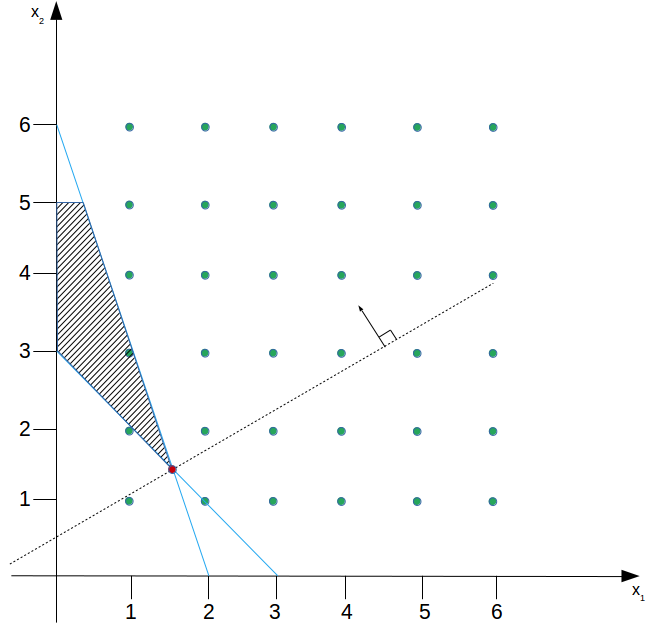
\includegraphics[height=12cm]{images/graph6.png}
	\label{fig:SoluzioneOttimaContinua1}
	\caption[]{\\Soluzione continua: $z=\frac{3}{4}$; $x_{1}=\frac{3}{2}$, $x_{2}=\frac{3}{2}$ \\ Soluzione intera: $z=4$; $x_{1}=1$, $x_{2}=2$}
\end{figure}

In questo esempio la soluzione arrotondata coincide con la soluzione ottima.

\begin{flalign}
& Es:\;\;Min\;z=8x_{1}+6x_{2} \\
& \;\;\;\;\;\;\;\;\;\;4x_{1}+3x_{2}\ge 6 \\
& \;\;\;\;\;\;\;\;\;\;x_{1},\;x_{2}\ge 0\;ed\;intere
\end{flalign}
\begin{figure}[h]
	\centering
	\captionsetup{justification=centering}
	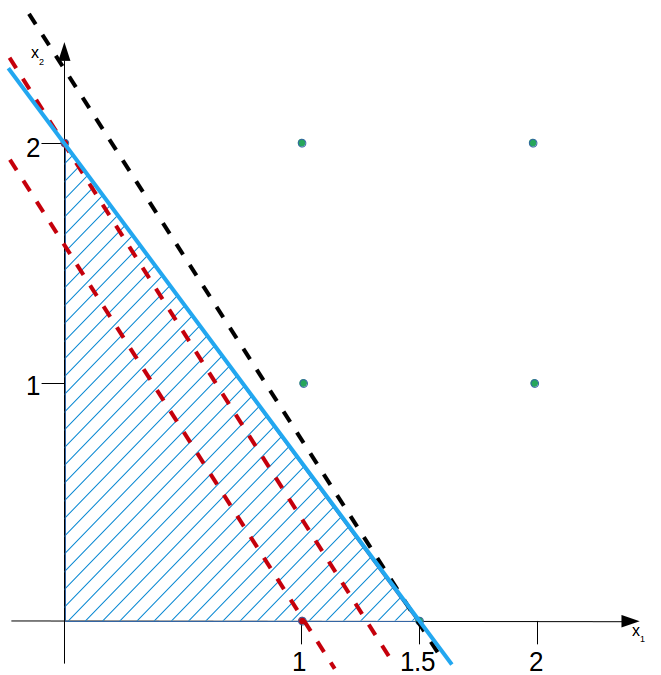
\includegraphics[height=13cm]{images/graph7.png}
	\label{fig:SoluzioneOttimaContinua2}
	\caption[]{\\ Soluzione continua: $z=12$; $x_{1}=1,5$, $x_{2}=0$ \\ Soluzione arrotondata $z=8$; $x_{1}=1$, $x_{2}=0$ \\ Soluzione intera: $z=10$; $x_{1}=0$, $x_{2}=2$}
\end{figure}

La soluzione arrotondata si discosta notevolmente dalla soluzione ottima.

\begin{flalign}
& Es:\;\;Min\;z=8x_{1}+6x_{2} \\
& \;\;\;\;\;\;\;\;\;\;4x_{1}+3x_{2}\ge 6 \\
& \;\;\;\;\;\;\;\;\;\;x_{1},\;x_{2}\ge 0\;ed\;intere
\end{flalign}
\begin{figure}[h]
	\centering
	\captionsetup{justification=centering}
	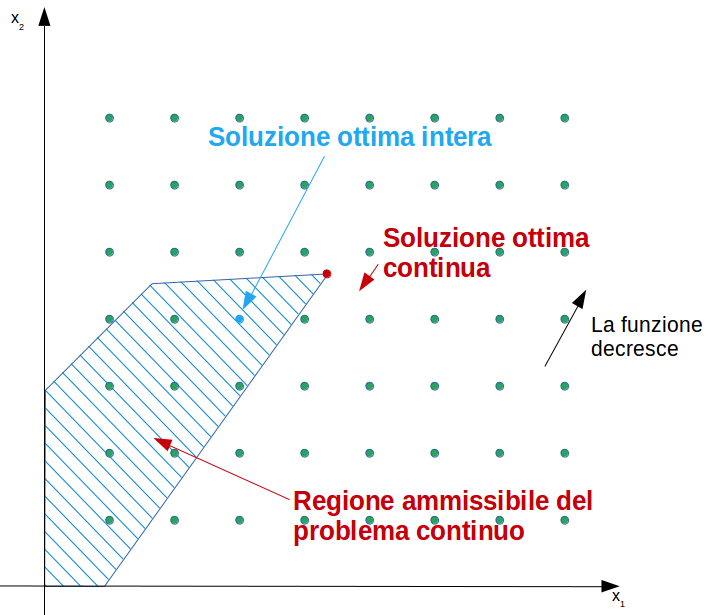
\includegraphics[height=14cm]{images/graph8.png}
	\label{fig:SoluzioneOttimaContinua3}
\end{figure}

I quattro punti interi pi\`u vicini alla soluzione continua non sono ammissibili.
\newpage

\section{Unimodularit\`a}
La matrice intera A di $m$ righe ed $n$ colonne \`e totalmente unimodulare se ogni sua sottomatrice quadrata B non singolare \`e unimodulare, ovvero $det(B)=\pm 1$.
\newline

\textbf{Teorema.} Se la matrice intera $A$ \`e totalmente unimodulare allora tutti i punti estremi dell'insieme pd. convesso $X={x:\;Ax=b,\;x\ge 0}$ sono interi per ogni vettore intero $b$.
\newline

\textbf{Dimostrazione.} Sia B una base ammissibile e $x_{b}$ le variabili base: $Bx_{B}=b$.\newline Per la regola di Cramer:
\begin{flalign}
	& x_{b_{i}}=\frac{\det(B_{i})}{\det(B)}
\end{flalign}
Dove $B_{i}$ si ottiene da $B$ sostituendo la i-esima colonna di $B$ con $b$. \`E ovvio che $\det(B_{i})$ \`e un numero intero e quindi anche ciascun $x_{B_{i}}$ \`e intero.
\newline

\textbf{Teorema.} Una matrice intera $A$ i cui elemento sono $0, +1, -1$ \`e totalmente unimodulare se:
\begin{enumerate}
	\item In ogni colonna $A$ compaiono al pi\`u due elementi non-nulli (cioè $1,-1$);
	\item L'insieme delle righe R pu\`o essere suddiviso in due insieme disgiunti $R_{1}$ e $R_{2}$ ($R_{1}\cup R_{2}=R$) per cui:
	\begin{enumerate}
		\item Se una colonna contiene due elementi non-nulli dello stesso segno allora la riga corrispondente ad uno dei due elementi appartiene a $R_{1}$ mentre la riga relativa all'altro elemento \`e in $R_{2}$;
		\item Se una colonna contiene due elementi di segno opposto entrambe le righe appartengono allo stesso insieme.
	\end{enumerate}
\end{enumerate}

\textbf{Esempi.}
\newline

\begin{tabular}{cc}
	$ A=\begin{bmatrix}
		-1 & 1 & 1 & 0 & 0 & 0 \\
		0 & 0 & -1 & -1 & 1 & 1 \\
		0 & 0 & 0 & 0 & 0 & -1 \\
		1 & -1 & 0 & 1 & -1 & 0 \\
	\end{bmatrix},$ &
	$A = \begin{bmatrix}
		-1 & 1 & 1 & 0 & 0 & 0 \\
		0 & 0 & -1 & -1 & 1 & 1 \\
		0 & 0 & 0 & 0 & 0 & -1 \\
		1 & -1 & 0 & 1 & -1 & 0 \\
	\end{bmatrix}$ \\
	\begin{minipage}{0pt}
		\vskip 10pt
		\begin{itemize}
			\item[$R={1,2,3,4}$]
			\item[$R_{1}={1,2,3,4}$]
			\vspace{-6mm}
			\item[$R_{2}=\emptyset$]
			\vspace{-6mm}
		\end{itemize}
	\end{minipage} &
	\begin{minipage}{0pt}
		\vskip 10pt
		\begin{itemize}
			\item[$R={1,2,3,4,5}$]
			\item[$R_{1}={1,2,3}$]
			\vspace{-6mm}
			\item[$R_{2}={4,5}$]
			\vspace{-6mm}
		\end{itemize}
	\end{minipage} \\
\end{tabular}

La totale unimodularit\`a della matrice $A$ \`e \textbf{condizione sufficiente} affinch\`e la soluzione ottima $x^{*}$ sia intera per
\begin{flalign*}
	& Min\;cx\\
	& \;\;\;\;\;\;\;\;Ax=b\;(b intero)\\
	& \;\;\;\;\;\;\;\;x\ge 0
\end{flalign*}
La condizione non \`e \textbf{necessaria}.\newline\newline
\textbf{Esempio:}

dato il sistema di vincoli
\begin{flalign*}
	& 6x_{1}+x_{2}=7 \\
	& 2x_{1}+x_{2}=3
\end{flalign*}
L'unica soluzione \`e ($x_{1}=1,\;x_{2}=1$) mentre la matrice
\begin{center}
	$ A=\begin{bmatrix}
	6 & 1 \\
	2 & 1
	\end{bmatrix}$	
\end{center}
non risulta essere totalmente unimodulare.
